\documentclass{article}
\documentclass[12pt]{document}
\usepackage[utf8]{inputenc}
\usepackage[spanish]{babel}
\usepackage{graphicx}
\title{      
\includegraphics[scale=0.5]{logo-universidad-de-antioquia.png}

GRANDES PENSADORES QUE DIERON VIDA A LA COMPUTACIÓN MODERNA}
\author{Juan Diego Sánchez Ramos
}

\date{\today}


\begin{document}



\maketitle 

Se expone de manera clara y precisa los sucesos que marcaron un antes y un después en la historia de la computación, también cómo se entrelazaron y complementaron conocimientos de grandes personajes que fueron esenciales para el desarrollo de esta historia

“La matemática debe mucho a David Hilbert. Fue una mente universal,  por tanto la Crisis de los Fundamentos atrajo su atención. Formuló un grandioso programa  el cual consistía, en primer lugar, en elaborar un método que permitiese construir la matemática en base a un conjunto de axiomas. Luego, se debe elaborar un método que pruebe la consistencia o inconsistencia de la teoría” (Ortíz, 1990). \cite{ortizcrisis}

Los veintitrés problemas que planteó Hilbert atrajeron a multitud de jóvenes investigadores a intentar dar solución a ellos, entre ellos Kurt Godel.Un estudiante de física teórica, que tras adentrarse al mundo de la lógica de Russell y asistir a las conferencias de David Hilbert sobre sus programas de completud y consistencia, decide cambiar el rumbo de su carrera y así estudiar lógica matemática.

Godel eligió el problema de Hilbert como tópico de investigación para su tesis doctoral.
En 1930 obtuvo el doctorado y su tesis fue publicada. Entonces enfocó su mirada en el programa de Hilbert, ese mismo año se dio cita a el congreso matemático, donde después de muchos años de debates intelectuales teniendo como tema principal si las matemáticas eran inquebrantables o no,  teniendo en cuenta que en el año 1874 el matemático conjuntista George Cantor había despertado una cantidad increíble de dudas al tocar el tan esquivo tema del infinito.
 
Solo un año después, en 1931 fue donde saltó a la fama y fue considerado el matemático más trascendental del siglo XX  con su obra “Sobre Proposiciones Indecidibles de los Principia Mathematica y sistemas afines” que contiene sus famosos teoremas de incompletitud  y que vino a dar respuesta al programa del célebre  Hilbert , demostrando que  era imposible de llevar a cabo, que siempre van a existir enunciados en los que no se pueda demostrar su veracidad o falsedad, dando así fin a la tan polémica “crisis de los fundamentos” La explicación y desarrollo de los mismos es una de los logros más grandiosos de la mente humana y han sido suficientes para colocar a Godel a la altura de los genios como Aristóteles o Einstein y que acabó por revolucionar el estudio de los fundamentos.
 
Uno de los encargados de seguir con el legado de Godel, Alan Mathison Turing nacido el veintitrés de Junio de l912, brillante matemático, criptoanalista e informático teórico, graduado con honores de la Licenciatura en Matemáticas en 1934, penetró los dominios de las matemáticas superiores al resolver, de manera sorprendentemente sencilla, el Entscheidungsproblem (o tambièn “el problema de la decidibilidad”) planteado por el legendario matemático  David Hilbert. 
Para llevar a cabo su demostración, usó lo que hoy conocemos como la Máquina de Turing, un modelo para muchos  sencillo el cual consiste de una cinta con longitud infinita dividida en cuadros en cada uno de los cuales podía colocarse un sólo símbolo. La máquina tiene básicamente 3 funciones, leer, escribir o borrar símbolos de la cinta, moviéndose para ello a razón de un cuadro a la vez .                                                                                                                                                                                                                                                                                                   \begin{figure}[h!]
\centering
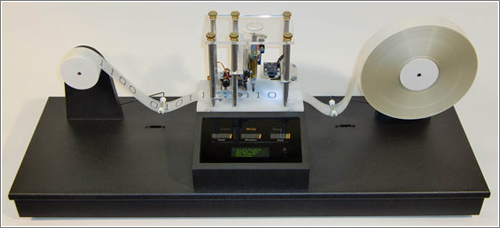
\includegraphics[scale=0.6]{turingFull560.jpg}
\caption{Máquina de Turing universal}
\label{fig:universe}
\end{figure}           

A pesar de que teóricamente era muy simple, esta máquina realmente estaba modelando un algoritmo y sería la primera herramienta teórica para explorar los límites de las computadoras. Las implicaciones de la demostración de Turing resultaron ser los orígenes de lo que hoy se conoce como teoría de la computación, y gracias a este trabajo sabemos en la actualidad que sin importar qué tan rápidas y poderosas puedan llegar a ser las computadoras que el hombre construya, aun así seguirán existiendo problemas que nunca podremos resolver. 
 
Por consiguiente, así es como Alan Mathison Turing, se convierte en el pionero de la computación y la teoría formal de algoritmos con sus aportaciones a esta. El cual siguiendo los trabajos de Godel y Hilbert, tuvo las bases teóricas suficientes para desarrollar su teoría.
Es curioso que los ordenadores que hoy en día conocemos y que son tan prácticos y necesarios para nuestra vida moderna, hayan sido resultado de una demostración para ayudar a  aclarar una de las más grandes dudas  relacionadas a los Fundamentos de las Matemáticas.
Cada uno de los personajes ya mencionados, fueron indispensables con sus aportes, conocimientos y correcciones para concebir una idea que en épocas remotas se consideraba irreal y es la esencia del funcionamiento de lo que ahora mismo llamamos ordenador. “(...) Cabe resaltar que los fracasos que tuvo Hilbert, fueron un gran éxito; no para el razonamiento o lógica matemática, sino para la programación,  el cálculo y la computación” (Gregory, 2003). \cite{chaitin2003ordenadores}


Todas las demás referencias bibliográficas : \cite{coello2003breve} \cite{ferreiros2004episodio} \cite{mathinfalibles} \cite{incytde}







\bibliographystyle{plain}
\bibliography{bibliografia.bib}

\end{document}